\chapter{Framework's architecture}
\label{chap:03}

At the highest macro level the framework can be put into perspective as shown in figure \ref{fig:architecture1}. 


\begin{figure}[h]
	\centering
	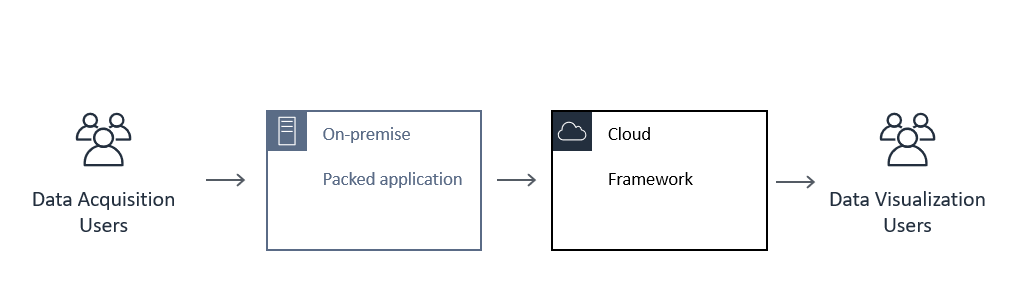
\includegraphics[width=1\linewidth]{./images/architecture/highest_lvl.png}
	\caption{Highest level of architecture view}
	\label{fig:architecture1}
\end{figure}

The roles and components are:
\begin{itemize}
	\item Data acquisition users -  these are external users that get data from any source and have the responsibility to wrap the fetching into an application and use the framework to upload it
	\item Packed application - the application made on-premise by the data acquisition user
	\item Framework - a web application hosted in cloud, used for uploading the packed application and also to visualize its output
	\item Data visualization users - the beneficiaries of the wrapped application, they can visualize information with the help of plots
\end{itemize}

\begin{figure}[h]
	\centering
	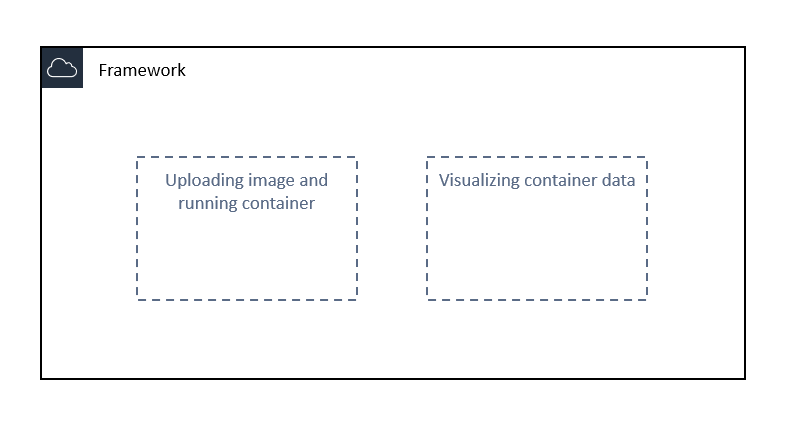
\includegraphics[width=1\linewidth]{./images/architecture/framework.png}
	\caption{Framework's main components}
	\label{fig:architecture2}
\end{figure}

Figure \ref{fig:architecture2} zooms in the Framework components. The two blocks are as follows:
\begin{itemize}
	\item Uploading image and running containers - the data acquisition user after wrapping his fetching data application can use this side of the web application to upload and run it. The steps of achieving this goal is further discussed in \autoref{chap:04}.
	\item Visualizing container data - this side of the framework is a tool which can be used to select plots filled with data coming from containers. Selection and usage of these plots is discussed in depth at \autoref{chap:04}.
\end{itemize}

